\section{Examples}
\subsection{Equations}
\[
  f(x) = 
    \underbrace{(x + 2)^3}_\text{text 1} + 
    \bigl(
      \mathrlap{\overbrace{\phantom{(c - 2d)}}^{\text{text 2}}}
      (c - 
      \mathrlap{\underbrace{\phantom{2d) + (3e}}_{\text{text 3}}}
      2d) +
      \overbrace{(3e - 4f)}^{\text{text 4}}
    \bigr) + 
    \overbrace{(x - 3)}^\text{text 5}
\]

$$\begin{vmatrix}
	\lambda -1 		& 0 				& 0				\\
	0 				& \lambda -2		& 0				\\
	0 				& 0 				& \lambda-3		\\
	\end{vmatrix}
=(\lambda-1)(\lambda-2)(\lambda-3)=0$$

\begin{equation*}
	\Big\|\sum_{i=1}^na_i(e_i-v_i)\Big\|^2=\,\Big\langle \sum_{i=1}^n a_i(e_i-v_i),\sum_{j=1}^n a_j(e_j-v_j)\Big\rangle
\end{equation*} 

\begin{equation} 
    \begin{split} 
    c_{11}& = a_{11}b_{11}+\dots+a_{1n}b_{n1}\\
    c_{22}&= a_{21} b_{12} +\dots+a_{2n} b_{n2} \\
    &\vdots\\
    c_{nn} & = a_{n1} b_{1n} +\dots+a_{nn}b_{nn}
    \end{split} 
\end{equation} 

\[
	e_3=\Big|\Big|x^2-x+\dfrac{1}{6}\Big|\Big|=\sqrt{\displaystyle \int_{0}^{1}\Big(x^2-x+\dfrac{1}{6}\Big)dx}=\sqrt{\dfrac{1}{180}}=\dfrac{1}{6\sqrt{5}}
\]

$$\lim_{x \to \infty}p(x) = \lim_{x \to -\infty}p(x) = \infty$$

\[
	f(x,y) =
	\begin{cases} 
		\frac{x^4 - y^4}{(x^2 + y^2)^2} & (x,y) \neq 0 \\
		b 								& (x,y) = 0
	\end{cases}
\]

\[
\lim_{(x,y)\to(0,0)}\frac{x^4-y^4}{(x^2+y^2)^2}
\]

$$
	D_F (x,y,z)=
	\begin{bmatrix}
		\frac{\partial f}{\partial x} & \frac{\partial f}{\partial y} & \frac{\partial f}{\partial z}\\
		\frac{\partial g}{\partial x} & \frac{\partial g}{\partial y} & \frac{\partial g}{\partial z}\\
		\frac{\partial (f+g)}{\partial x} & \frac{\partial (f+g)}{\partial y} & \frac{\partial (f+g)}{\partial z}\\
	\end{bmatrix}
$$

\begin{align*}
	f(x_1,x_2)  &= x_1e^{-x_2} + x_2 + 1, x_0\\
	f_{x_1}(x_1,x_2) &= e^{-x_2},  \\
	f_{x_2}(x_1,x_2) &= -x_1e^{-x_2} +1  \\
	f_{{x_1}{x_1}}(x_1,x_2) &= 0  \\
	f_{{x_1}{x_2}}(x_1,x_2) &= -e^{-x_2}  \\
	f_{{x_2}{x_2}}(x_1,x_2) &= x_1e^{-x_2}  
\end{align*}

\[
	\begin{bmatrix}
		1 & 0 & \hdots & 0 & 0 \\
		-a & 1 & \ddots & \ddots & 0 \\
		0 & -a & 1 & \ddots & 0 \\
		\vdots & \vdots & \ddots & \ddots	 & \vdots \\
		0 & 0 & 0 & -a & 1 
	\end{bmatrix}
	\begin{bmatrix}
		y_1 \\
		y_2 \\
		\vdots \\
		y_n 
	\end{bmatrix} 
	=
	b
	\begin{bmatrix}
		u_1 \\
		u_2 \\
		\vdots \\
		u_n 
	\end{bmatrix}
	+
	\begin{bmatrix}
		v_1 \\
		v_2 \\
		\vdots \\
		v_n 
	\end{bmatrix}
\]

\begin{equation*}
	\frac{\partial^2T}{\partial x^2}\Bigg\vert_{m,n} = \frac{\partial T/\partial x\vert_{m+1/2,n}-\partial T/\partial x\vert_{m-1/2,n}}{\Delta x}
\end{equation*}

\begin{multline*}
p(x) = 3x^6 + 14x^5y + 590x^4y^2 + 19x^3y^3- 12x^2y^4 - 12xy^5 + 2y^6 - a^3b^3 - 12x^2y^4 - 12xy^5 + 2y^6 - a^3b^3 \\ 
- 12x^2y^4 - 12xy^5 + 2y^6 - a^3b^3
\end{multline*}

\newpage
\subsection{Figures}

The following figures are just to show the positioning and sizing. They are not sized properly.

\begin{figure}[H] % H is used due to float package. Others: h: here, t: top, b: bottom, p: page of float
	\centering
	\subfloat[Bode gain.]{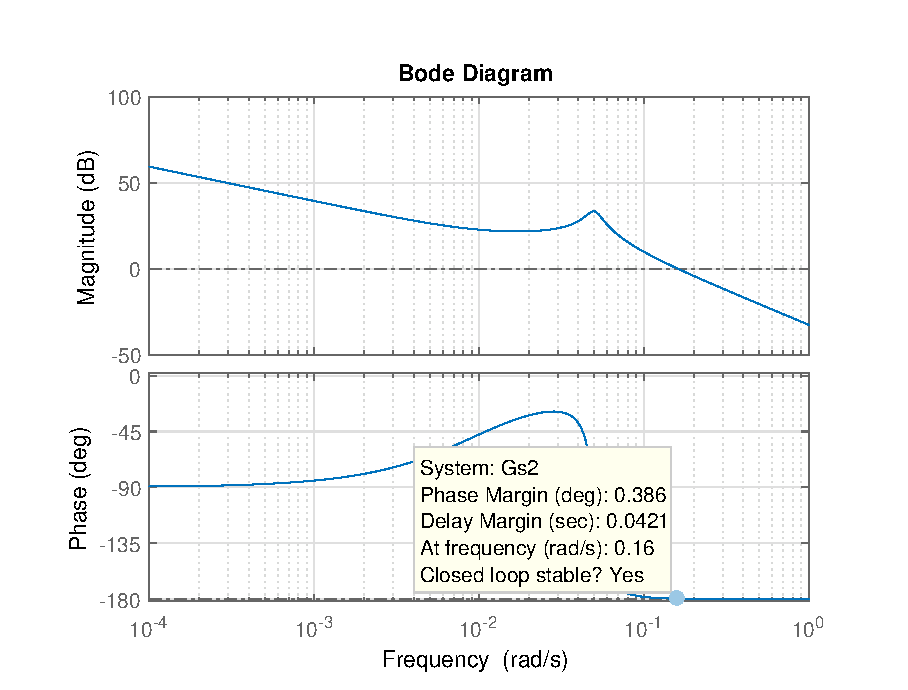
\includegraphics[width=0.5\textwidth]{./fig/Q5_B_Bode_Gained.eps}\label{fig:Q5_B_Bode_Gained}}
	\hfill
	\subfloat[Step response.]{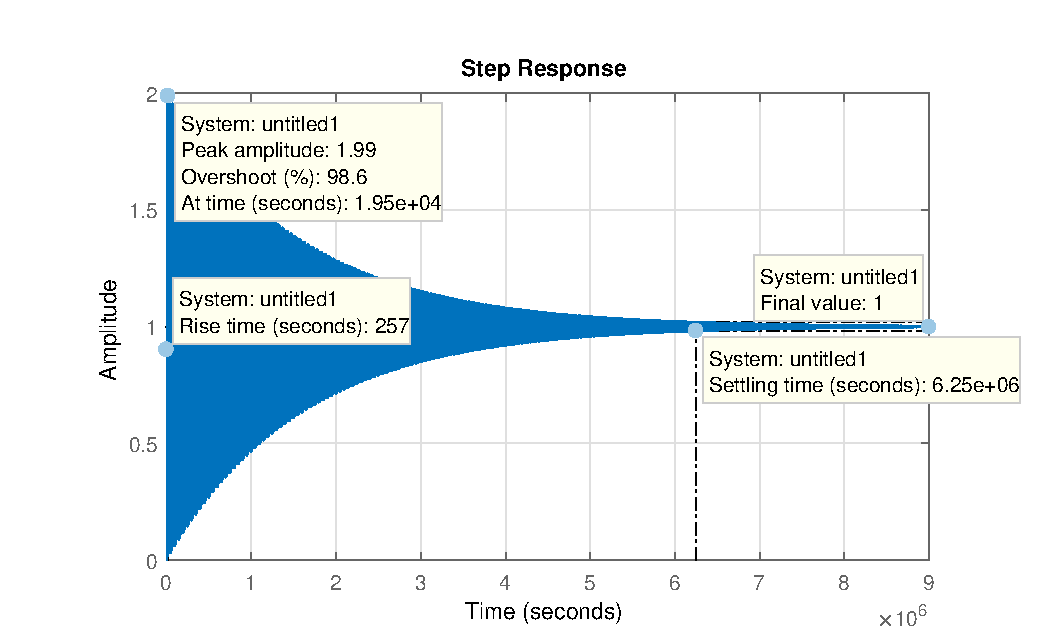
\includegraphics[width=0.5\textwidth]{./fig/Q5_G_step.eps}\label{fig:42}}
	\caption{Control plots.}
\end{figure}

\begin{figure}[H]  % H is used due to float package. Others: h: here, t: top, b: bottom, p: page of float
	\centering
	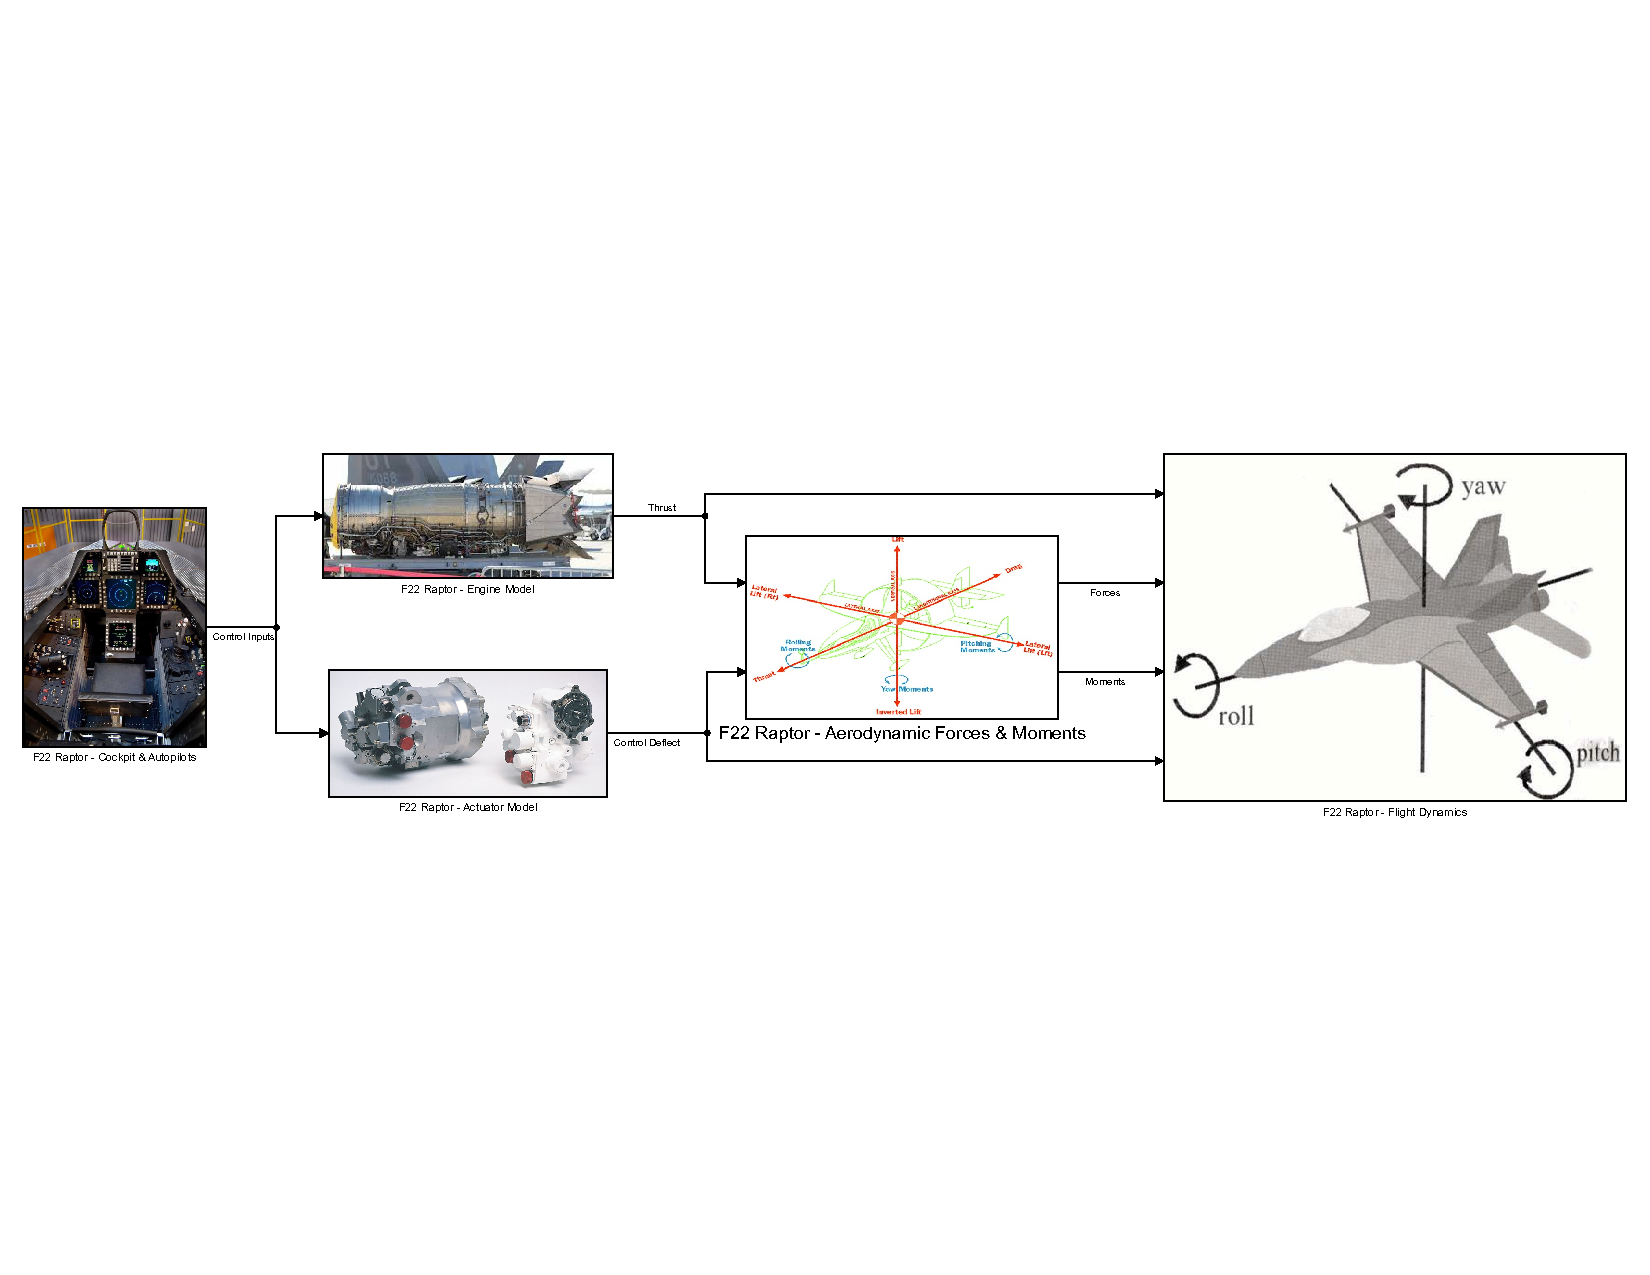
\includegraphics[trim={0 7.5cm 0 7.5cm},clip,width=\linewidth]{./fig/00_F22_Model_v2}
	% trim={<left> <lower> <right> <upper>}
	\caption{Simulink block that has the environment model}
	\label{00F22Model} 
\end{figure}

\begin{figure}[H]  % H is used due to float package. Others: h: here, t: top, b: bottom, p: page of float
	\centering	
	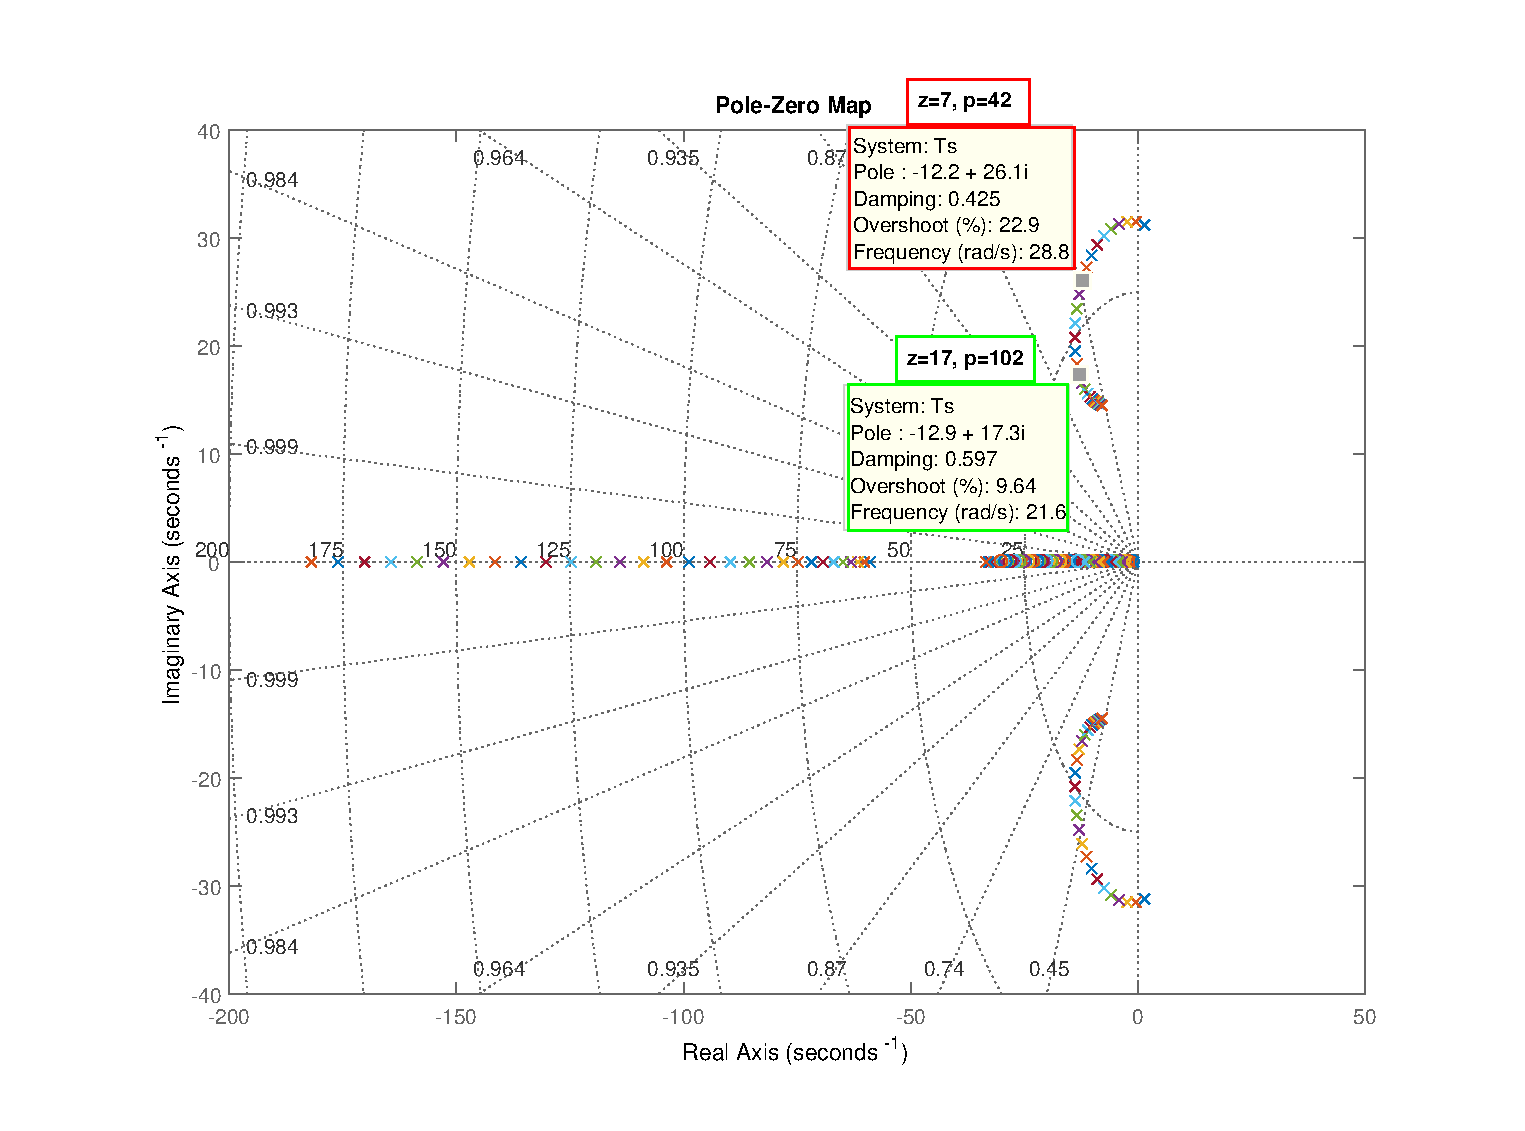
\includegraphics[width=\linewidth]{./fig/Q01_A_pzmap.eps}
	% trim={<left> <lower> <right> <upper>}
	\caption{Pole-Zero map of the closed-loop transfer function for different $z$ values}
	\label{fig:Q01_A_pzmap} 
\end{figure}

\subsection{Tables}

Create tables on \href{https://www.tablesgenerator.com/}{Latex Table Generator Website}. Or prepare in MS Office Excel and save as PDF file.

\begin{table}[H]  % H is used due to float package. Others: h: here, t: top, b: bottom, p: page of float
	\centering
	\caption{Permutation results}
	\label{tab:problem14}
	\begin{tabular}{|c|c|c|}
		\hline
		\textbf{System}  & \multicolumn{1}{l|}{\textbf{$K_p$}} & \multicolumn{1}{l|}{\textbf{$\omega_n$}} \\ \hline
		\multirow{4}{*}{$G_1(s)$} & 0                                   & 1                                \\ \cline{2-3} 
		& 0                                   & 1                                \\ \cline{2-3} 
		& 0                                   & 1                                \\ \cline{2-3} 
		& 0                                   & 1                                \\ \hline
	\end{tabular}
\end{table}